\chapter{Oscilador Armónico Cuántico}

\section{Problemas}

\begin{ejercicio}
\textbf{Full1: 1}
Ecuentra las expressiones del los observables $x$ y $p$ en términos de los
operadores $a$ y $a^\dagger$ que permiten escribir l'hamiltoniano armónico
unidimensional como $H = \hbar \omega (a^\dagger a + 1/2)$. Conviene que
utilizas argumentos d'hermitinidad y dimensional.	\\\\
\end{ejercicio}
\begin{solucion}
Los operadores escalera estan definida por
\begin{align*}
	a \,=\, \sqrt{\frac{m\omega}{2 \hbar}} \left( \hat x + \frac{i}{m \omega} \hat p
\right)	\\
	a^\dagger \,=\, \sqrt{\frac{m\omega}{2 \hbar}} \left( \hat x - \frac{i}{m \omega}
\hat p\right)
\end{align*}
Así añadiendo y sustraiendo los operadores escalar danos
\begin{align*}
	a + a^\dagger \,=\,a \sqrt{\frac{m \omega}{2 \hbar}} ( \hat x + \hat x) &
\Rightarrow \quad \hat x \,=\, \sqrt{\frac{\hbar }{2 m \omega}} (a + a^\dagger) \\
	a - a^\dagger \,=\,a \sqrt{\frac{m \omega}{2 \hbar}} \left(\frac{i}{m
\omega} \hat p + \frac{i}{m \omega} \hat p \right) a \Rightarrow \quad \hat p
\,=\, \sqrt{\frac{\hbar m \omega}{2}} (-i) (a - a^\dagger)
\end{align*}
Ahora vamos a comprobar la dimensionalidad. En general los unidades utilizados
para los operadores escalares estan
\begin{align*}
	m \,=\, kg \quad \omega \,=\, \sqrt{\frac{k}{m}} \,=\, \frac{1}{s} \quad h
\,=\, \frac{kg \cdot m^2}{s},
\end{align*}
porque $h = J\cdot s = N \cdot m \cdot s$ y $k = N / m = kg / s$. Así que la
comproba de $\hat x$
\begin{equation*}
	\hat x \,=\, \sqrt{\frac{h}{m \omega}} \,=\, \sqrt{\frac{kg \cdot m^2}{s} 
\cdot kg^{-1} \cdot s} \,=\, m
\end{equation*}
y de $\hat p$
\begin{equation*}
	\hat p \,=\, \sqrt{h m \omega} \,=\, \sqrt{\frac{kg \cdot m^2}{s} \cdot kg
\cdot s^{-1}} \,=\, \frac{kg \cdot m}{s}
\end{equation*}
donde hemos mirado solo términos importantes, estan hecho facilmente.

\end{solucion}
% -----------------------------------------------------------------------------


\begin{ejercicio}
\textbf{Full1: 2} Utilza los operadores escalar $a$ y $a^\dagger$ para calcular los valores
esperados $\langle x \rangle_n$, $\langle p \rangle_n$, $\langle x^2 \rangle_n$,
$\langle p^2 \rangle_n$, $\langle K \rangle_n$, $\langle V \rangle_n$ y los
indeterminaciónes $\langle (\Delta x)^2 \rangle_n$, $\langle(\Delta p)^2\rangle_n$ y
$\langle(\Delta H)^2\rangle_n$ de el estado
estacionario $|n\rangle$ de l'oscilador armónico unidimensional. 
\end{ejercicio}
\begin{solucion}
Recuerdando que los vectores del estado estan orthogonales
\begin{equation*}
	\langle n | n' \rangle \,=\, \delta_{nn'}
\end{equation*}
nos podemos calcular $\langle \hat x \rangle_n$ y $\langle \hat p \rangle_n$
facilmente 
\begin{align*}
	\langle \hat x \rangle_n a= \langle n | \hat x | n \rangle =
\sqrt{\frac{\hbar}{2m\omega}} \langle n| a^\dagger + a | n \rangle 
	= \sqrt{\frac{\hbar}{2m\omega}} (\langle n | a^\dagger | \rangle +
\langle n | a | n \rangle ) \\
	a = \sqrt{\frac{\hbar}{2m\omega}} (\sqrt{n+1} \langle
n| n+1\rangle + \sqrt{n} \langle n|n-1\rangle) = 0,\\
	\langle \hat p \rangle_n a= \sqrt{\frac{\hbar}{2m\omega}} (-i) \langle n |
(a - a^\dagger) | n \rangle = 0.
\end{align*}
Utilizando el operador número $N = a^\dagger a$ y el commutador de los
operadores escalar
\begin{equation*}
	[a, a^\dagger] = aa^\dagger - a^\dagger a = 1 \quad \Rightarrow \qquad a
a^\dagger = a^\dagger a + 1 = \hat N + 1	
\end{equation*}
danos las valores esperados de $\langle \hat x^2 \rangle_n$ y $\langle \hat p^2
\rangle_n$
\begin{align*}
	\langle \hat x^2 \rangle_n a= \langle n | \hat x^2 | n \rangle =
\frac{\hbar}{2m\omega} (\langle n | \cancel{a^\dagger a^\dagger} +
\underbrace{a^\dagger a}_{\hat N} + \underbrace{aa^\dagger}_{\hat N + 1} +
\cancel{aa} | n\rangle  \\
	a= \frac{\hbar}{2m\omega} (\langle n | 2 \hat N + 1 | n \rangle =
\frac{\hbar}{2m\omega} (2n +1) = \frac{\hbar}{m\omega}
\left(n+\frac{1}{2}\right) \\
	\langle \hat p^2 \rangle_n a= -\frac{\hbar m \omega}{2} [-(2n +1] =
\frac{\hbar m \omega}{2} (2n + 1) = \hbar m \omega (n + \frac{1}{2}).	
\end{align*}
Los valores esperados kintetico $\langle K \rangle_n$ y potencial $\langle V
\rangle_n$ estan compuesto de los valores esperados calculado antes, por lo
tanto nos podemos escribir
\begin{align*}
	\langle K \rangle_n a= \frac{1}{2m} \langle \hat p^2 \rangle_n \frac{\hbar
\omega}{2} \left( n \frac{1}{2} \right) \\
	\langle V \rangle_n a=  \frac{1}{2} m \omega^2 \langle x^2 \rangle_n =
\frac{1}{2} \hbar \omega \left( n + \frac{1}{2} \right)
\end{align*}
Por esto $\langle H \rangle_n$  esta dado por
\begin{equation*}
	\langle H \rangle_n = \langle K \rangle_n + \langle V \rangle_n = \hbar
\omega \left( n + \frac{1}{2} \right).
\end{equation*}
Por los indeterminaviones nos recuerdamos de la relación de indeterminación
\begin{equation*}
	\Delta A \equiv A - \langle A \rangle \quad \Rightarrow \qquad \langle
(\Delta A)^2 \rangle = \langle A^2 \rangle - \langle A \rangle^2
\end{equation*}
Así los indeterminaciones estan dado por
\begin{align*}
	\langle (\Delta x)^2 \rangle_n a= \langle x^2 \rangle_n -
\underbrace{\langle x \rangle_n}_0 = \frac{\hbar}{m\omega} \left( n +
\frac{1}{2}\right) \\
	\langle (\Delta p)^2 \rangle_n a= \langle p^2 \rangle_n -
\underbrace{\langle p \rangle_n}_0 = \hbar m \omega \left(n + \frac{1}{2}
\right) \\
	\langle (\Delta H)^2 \rangle_n = \langle H^2 \rangle_n - \langle H
\rangle_n^2 = 0
\end{align*}
El ultimo realción esta verdad porque dando un Hamiltoniano armónico
\begin{equation*}
	H = \frac{1}{2m} p^2 + \frac{1}{2} m \omega^2 x^2 \quad \Rightarrow \qquad
H^2 = \frac{1}{4m^2} \underbrace{p^4}_{(a-a^\dagger)^4} + \frac{1}{4} m^2
\omega^2 \underbrace{x^4}_{(a+a^\dagger)^4}
\end{equation*}
así considerado solo $x^4$
\begin{equation*}
	\langle x^4 \rangle_n = \langle n |(a+a^\dagger)^4 | n \rangle = \langle n |(\cancel{aa} + aa^\dagger + a^\dagger a + \cancel{a^\dagger
a^\dagger})^2 | n \rangle = \langle n |(aa^\dagger + a^\dagger a)^2 | n \rangle
= \langle n | ( a a^\dagger + a^\dagger a) | n \rangle^2  
\end{equation*}
repitiendo el mismo processo por $p^4$ danos como resultado
\begin{equation*}
	\langle H^2 \rangle_n = \langle H \rangle_n^2
\end{equation*}
por lo tanto vemos que la indeterminacion del Hamiltoniano esta cero.
\end{solucion}
% -----------------------------------------------------------------------------


\begin{ejercicio}
\textbf{Full1: 3} 
Por el estado no estacionario inicial (y sencillo) $|\psi(t=0)\rangle =
\frac{1}{\sqrt{2}} |0\rangle + \frac{1}{\sqrt{2}} | 1 \rangle$ y cualquier
instant de tiempo t. 
\end{ejercicio}
\begin{solucion}
Primero tenemos que evaluar la evolución del tiempo del estado no esacionario
inicial. Por lo tanto deberiamos calcular la energía del oscillador armónico
del estado fundamental y primero estado
\begin{equation*}
	E_n = \hbar \omega (n + \frac{1}{2}), \quad E_0 = \frac{\hbar \omega}{2}
,\quad E_1 = \frac{3 \hbar \omega}{2}.
\end{equation*}
Así utilizando
\begin{equation*}
	|\alpha (t)\rangle = \sum_n \alpha_n e^{-i\frac{E_n}{\hbar} t} | n\rangle
\end{equation*}
danos la evolución temporal de $|\psi(t=0)\rangle$ 
\begin{equation*}
	|\psi(t)\rangle = \frac{1}{\sqrt{2}} e^{-\frac{i\omega}{2}}|0\rangle
+ \frac{1}{\sqrt{2}} e^{-\frac{3 i \omega t}{2}} |1 \rangle  = \frac{1}{\sqrt{2}}
e^{-\frac{i\omega t}{2}} \left( |0\rangle + e^{\frac{i \omega t}{2}} |
2\rangle \right)
\end{equation*}
Logicamente por los valores eseperados nos tenemos
\begin{align*}
	\langle \hat x \rangle_{\psi(t)} &= \langle \psi | \hat x | \psi \rangle \\
	&= \frac{1}{2} \cancel{e^{\frac{- i \omega t}{2}}e^{\frac{i \omega t}{2}}}
\frac{\hbar}{2m\omega} \left( \langle 0| + e^{i\omega t} \langle 1 | \right) ( a +
a^\dagger) \left( e^{i\omega t} | 1 \rangle + | 0 \rangle \right) \\
	&= \frac{1}{2} \sqrt{\frac{\hbar}{2m\omega}} \left( e^{-i\omega t}\langle 0
| a | 1 \rangle + e^{i\omega t} \langle 1 | a^\dagger | 0 \rangle \right) \\
	&= \frac{1}{2} \sqrt{\frac{\hbar}{2m\omega}} \left( e^{-i\omega t} + e^{i
\omega t} \right) \\
	&= \frac{1}{2} \sqrt{\frac{\hbar}{2m\omega}} \cos{\omega t}  
\end{align*}
y 
\begin{align*}
	\langle \hat p \rangle_{\psi(t)} &= \frac{1}{2} \sqrt{\frac{\hbar m
\omega}{2}} (-i) \left( \langle 0| + e^{i\omega t} \langle 1| \right) (a -
a^\dagger) \left( e^{-i\omega t} |1\rangle + |0\rangle \right) \\
	&= \frac{1}{2} \sqrt{\frac{\hbar m \omega}{2}} (-i) \left( e^{-i\omega
t}\langle 0 | a | 1 \rangle - e^{i\omega t} \langle 1| a^\dagger | 0 \rangle
\right) \\
	&= \sqrt{\frac{\hbar m \omega}{2}} \frac{1}{2i}\left( e^{-i\omega t} -
e^{i \omega t} \right) \\
	&= -\sqrt{\frac{\hbar m \omega}{2}} \sin{\omega t}  
\end{align*}
\end{solucion}
% -----------------------------------------------------------------------------


\begin{ejercicio}
\textbf{Full1: 4}
Dada la function d'onda del estado fundamental del oscilador armónico
unidimenional
\begin{equation*}
	\phi_0 (x) = \left(\frac{m\omega}{\pi \hbar}\right)^{\frac{1}{4}} e^{-\frac{1}{2}
\frac{m\omega}{\hbar} x^2}
\end{equation*}
ecuentre l'expresion de $\phi_2(x)$. 
\end{ejercicio}
\begin{solucion}
Nos podemos escribir el operador escalar $a^\dagger$ en la siguiente forma
\begin{equation*}
	a^\dagger = \frac{1}{\sqrt{2\hbar m\omega}}(m \omega \hat x - i \hat p) \quad
\text{con} \quad a^\dagger | n \rangle = \sqrt{n+1} | n+1 \rangle
\end{equation*}
Así
\begin{equation*}
	(a^\dagger )^2 | 0 \rangle = \sqrt{1} a^\dagger | 1 \rangle = \sqrt{2} | 2
\rangle \quad \Rightarrow \qquad | 2\rangle = \frac{1}{\sqrt{2}}(a^\dagger)^2 | 0 \rangle
\end{equation*}
y por lo tanto $\phi_2 (x)$ esta dado por
\begin{equation*}
	|2\rangle = \phi_2 = \frac{1}{\sqrt{2}} \phi_0.
\end{equation*}
Empezando con el operador escalar cuadrado
\begin{equation*}
	(a^\dagger )^2 = \frac{1}{2\hbar m \omega} (m \omega \hat x - i \hat p)^2 =
\frac{1}{2\hbar m \omega} \left(m \omega \hat x - \hbar \frac{\partial}{\partial
x}\right)^2 = \frac{1}{2\hbar m \omega} \left(m^2 \omega^2 x^2 + \hbar
\frac{\partial^2}{\partial x^2} - 2 m \omega \hbar x \frac{\partial}{\partial
x}\right)
\end{equation*}
donde hemos utilizado el operador momento $\hat p = - i \hbar \partial/\partial
x$. Antes de continuar queremos caclular la segunda derivada de 
\begin{equation*}
	\frac{\partial^2}{\partial x^2} \left(e^{-\frac{1}{2} \frac{m\omega}{\hbar}
x^2}\right) = \frac{\partial}{\partial x} \left(\frac{m \omega}{\hbar} x \right)
e^{-\frac{1}{2} \frac{m\omega}{\hbar} x^2} = \left(-\frac{m\omega}{\hbar} +
\frac{m^2\omega^2}{\hbar^2}x^2\right) e^{-\frac{1}{2}\frac{m\omega}{\hbar} x^2}
\end{equation*}
Por lo tanto $\phi_2$ esta dado por
\begin{align*}
	\phi_2 &= \frac{1}{\sqrt{2}} \frac{1}{2 \hbar m \omega}
\left(\frac{m\omega}{\pi\hbar}\right)^{\frac{1}{4}} \left(m^2 \omega^2 x^2 +
\hbar^2 \frac{\partial^2}{\partial x^2} - 2m\omega\hbar x
\frac{\partial}{\partial x} \right) e^{\frac{1}{2} \frac{m\omega}{\hbar}x^2} \\
	&= \frac{1}{\sqrt{2}} \frac{1}{2\hbar m\omega}
\left(\frac{m\omega}{\pi\hbar}\right)^{\frac{1}{4}} \left(m^2 \omega^2 x^2 + 2
m^2 \omega^2 x^2 - m \omega \hbar + m \omega \hbar + m^2 \omega^2 x^2 \right)
e^{\frac{1}{2} \frac{m \omega}{\hbar} x^2} \\
	&= \left(\frac{m\omega}{\pi\hbar}\right)^{\frac{1}{4}}
\left(-\frac{1}{\sqrt{8}} + \sqrt{2} \frac{m\omega}{\hbar} x^2 \right)
e^{\frac{1}{2} \frac{m\omega}{\hbar} x^2}
\end{align*}
\end{solucion}
% -----------------------------------------------------------------------------

\begin{ejercicio}
	\textbf{Full1: 7} En la mecánica matricial, qual es el ket $|x =0 \rangle$ que represente un
oscilador situada exactamente al origen $x=0$? Distinguie entre componentes
pares y impares. Compara con los resultados de mecánica ondulatòria.
\end{ejercicio}
Aplicar el operador $\hat x$ al eigenket $|x=0\rangle$ logigamente danos
$$
	\hat | x=0 \rangle \overset{!}{=} 0 \quad \Rightarrow \qquad \hat x |
x=0\rangle = \sqrt{\frac{\hbar}{2 m\omega}} ( \hat a + \hat a^\dagger) | x = 0 \rangle = 0 
$$
En la forma del matrix podemos escribir los operadores escalar como
$$
	\hat a = \begin{pmatrix} 
	0 & 1 & 0 & 0 & \cdots \\
	0 & 0 & \sqrt 2 & 0 & \cdots \\
	0 & 0 & 0 & \sqrt 3 & \cdots \\
	0 & 0 & 0 & 0 & \cdots\\
	\cdots & \cdots & \cdots & \cdots & \cdots  
	\end{pmatrix}, \qquad \hat a^\dagger = \begin{pmatrix}
	0 & 0 & 0 & 0 & \cdots \\
	1 & 0 & 0 & 0 & \cdots \\
	0 & \sqrt 2 & 0 & 0 & \cdots \\
	0 & 0 & \sqrt 3 & 0 & \cdots \\
	0 & 0 & 0 & \sqrt 4 & \cdots \\
	\cdots & \cdots & \cdots & \cdots & \cdots  
	\end{pmatrix}
$$
Por lo tanto la suma esta dado por
$$
	(\hat a + \hat a^\dagger) |x=0\rangle = \begin{pmatrix}
	0 & 1 & 0 & 0 & 0 & \cdots \\
	1 & 0 & \sqrt 2 & 0 & 0 & \cdots \\
	0 & \sqrt 2 & 0 & \sqrt 3 & 0 & \cdots \\
	0 & 0 & \sqrt 3 & 0 & \sqrt 4 & \cdots \\
	0 & 0 & 0 & \sqrt 4 & 0 & \cdots \\
	\cdots & \cdots & \cdots & \cdots & \cdots  
	\end{pmatrix} \cdot \begin{pmatrix}
	c_0 \\ c_1 \\ c_2 \\ c_3 \\ c_4 \\ \vdots \\ c_n
	\end{pmatrix} = 0
$$
Ya tenemos un systema de ecuaciónes que podemos resolvar por los coeficientes
$c_n$
\begin{align*}
	c_1 = 0, \quad c_0 + \sqrt 2 c_2 = 0, \quad  \sqrt 2 c_2 + c_3 = 0, \quad
\sqrt 3 c_2 + \sqrt 4 c_4 = 0
\end{align*}
en consecuencia todo los $c_n$ con un index impar estan zero
$$
	c_{n+1} = 0 \quad \text{con} \qquad n \in 1, 2, 3, \cdots
$$
De hecho el systema de ecuaciónes danos por los $c_n$ con un index par 
$$
	c_2 = \frac{-c_0}{\sqrt 2}, \quad c_4 = - \frac{\sqrt 3}{\sqrt 4}c_2 =
\frac{3}{8}c_0, \quad c_6 = \frac{\sqrt{15}}{\sqrt{48}} c_0, \quad
\cdots
$$
Ademas, para encontrar la solution que obadece la mecanica cuantica, tenemos que
normalizar el eigenket con la introdución de un factor der normalización $N$.
Como podemos ver todos los coeficientes $c_n$ con un index par dependen de $c_0$
entonces solo tenemos que normalizarlo
$$ 
	\frac{c_0}{N} = 1
$$ 
y el resto esta dado por
$$
	\langle x = 0| x = 0\rangle = 1 \quad \Rightarrow \qquad | x=0 \rangle = N
\begin{pmatrix}
	1 \\ 0 \\ - \frac{1}{\sqrt 2} \\ 0 \\ \left(-\frac{1}{\sqrt
2}\right)\left(-\frac{\sqrt 3}{\sqrt 4}\right) \\ \vdots  
	\end{pmatrix}.
$$
El eigenket $|x=0\rangle$ corresponde a una serie dado por
$$
	\frac{1}{N} C_2n = (-)^n \sqrt{\frac{(2n-1)!!}{2^n n!}}
$$
\red{normalization problem}
	
\rule{\textwidth}{1pt}

% ------------------------------------------------------------------------------------------
	
	
\begin{ejercicio}
\textbf{Full1: 10} Un estado coherente a $t=0$ esta dado por el ket
$$
	| \alpha_0 \rangle e^{\frac{1}{2} |\alpha_0|^2} \sum_{n=0}^{\infty}
	\frac{\alpha_0^n}{\sqrt{n!}} |n\rangle 
$$
Ecuentre el ket $|\alpha(t)\rangle$ que da su evolución temporal y comproba que
satisfará la equación de Schrödinger dependiendo de t. \\\\
\end{ejercicio}
Empezando por lo evolución temporal nos sabemos que los estados del oscilador
armónico esta dado por
$$	
	|n\rangle \overset{t}{\longrightarrow} e^{-i\frac{E_n}{\hbar}t} |n\rangle
\quad \Rightarrow \qquad |n\rangle \overset{t}{\longrightarrow} e^{i\omega(n +
\frac{1}{2}) t} |n\rangle
$$
Así el evolución temporal de $|\alpha_0\rangle$ esta dado por
$$
	|\alpha_0\rangle \overset{t}{\longrightarrow} |\alpha(t) \rangle =
e^{-\frac{1}{2} |\alpha_0|^2} e^{-\frac{i\omega t}{2}} \sum_{n=0}^{\infty}
\frac{\alpha_0^n}{\sqrt{n!}} e^{i\omega n t} |n\rangle.
$$
Para comprobar el ecuación de Schrödinger
$$
	i \hbar \frac{d}{dt} |\alpha(t) \rangle = H | \alpha(t) \rangle
$$
necesitamos de recuerdarnos de el operador de número
$$
	\hat N | n \rangle = a^\dagger a | n\rangle = n | n \rangle
$$ 
Por lo tanto 
\begin{align*}
	i \hbar \frac{d}{dt} |\alpha(t) \rangle &= i \hbar
\frac{d}{dt} \left(e^{-\frac{1}{2} |\alpha_0|^2} e^{-\frac{i \omega t}{2}} \sum_{n=0}^{\infty}
\frac{\alpha_0^n}{\sqrt{n!}} e^{-i\omega n t} | n\rangle \right) \\
	&= \frac{\hbar \omega}{2} \underbrace{e^{-\frac{1}{2}|\alpha_0|^2}
e^{-i\frac{i \omega t}{2}} \sum_{n=0}^\infty \frac{\alpha_0^n}{\sqrt{n!}}
e^{-i\omega n t} | n\rangle}_{|\alpha(t)\rangle} + \underbrace{\hbar \omega
e^{-\frac{1}{2} |\alpha_0|} e^{-\frac{i\omega t}{2}} \sum_{n=0}^\infty n
\frac{\alpha_0^n}{\sqrt{n!}}|n\rangle}_{\hat N | \alpha(t) \rangle}  \\
	&= \hbar \omega \left(\frac{1}{2} + a^\dagger a \right) |\alpha(t)\rangle = H | \alpha(t) \rangle
\end{align*}
\rule{\textwidth}{1pt}
%----------------------------------------------------------------------------------------------------


\begin{ejercicio}
\textbf{Full1bis: 1} 
Ultilza la regla de commutación $[a, a^\dagger] = 1$, comprobar que 
$$
	[a, (a^\dagger)^n] = n (a^\dagger)^{n-1} \quad  \text{y} \qquad [a^n,
a^\dagger] = n a^{n-1}.
$$
Ademas con los primeros resultatos justifica los relaciónes
$$	
	[a, f(a^\dagger)] = \frac{d f(a\dagger)}{d a^\dagger} \quad \text{y} \qquad [f(a),
	a^\dagger] = \frac{d f(a)}{d a}
$$
\end{ejercicio}
\begin{solucion}
Para derivar la premiero relación tenemos que utilizar la indución mathematica.
Empezando por la \textbf{iniciación de la inducción}
\begin{proof}
$$
	[a, (a^\dagger)^n] \overset{n=1}{=} [a, a^\dagger] = 1 \cdot (a^\dagger)^0 =
1 
$$
Ahora por demonstar el \textbf{paso inductive} utilizamos como
\textbf{hipótesis inductiva} la siguinte relacion
$$
	[a, (a^\dagger)^k] = k (a^\dagger)^{k-1}.
$$
Por lo tanto tenemos que comprobar que
$$
	[a, (a^\dagger)^{k+1}] \overset{!}{=} (k+1) (a^\dagger)^{(k)}
$$
Así, utilizando la hipótesis inductiva,
\begin{align*}
	[a, a^\dagger (a^\dagger)^k] &= [a, a^\dagger] (a^\dagger)^k + a^\dagger [a,
(a^\dagger)^k] \\
	&= (a^\dagger)^k + a^\dagger k (a^\dagger)^{k-1} \\
	&= (k+1)(a^\dagger)^k \qedhere
\end{align*}
\end{proof}
\begin{proof}
Por la segunda relación vamos a utilizar el mismo conzepto de indución
$$
	[a^n, a^\dagger] \overset{!}{=} n a^{n-1}
$$
mathematica. Así la \textbf{iniciación de la inducción} esta dado por
$$
	[a^1, a^\dagger] = 1 \cdot a^0 = 1
$$
y aplicar la \textbf{hiótesis inductiva} 
$$
	[a^k, a^\dagger] = k a^{k-1}
$$
danos la comporbación
\begin{align*}
	[a^{k+1}, a^\dagger] &\overset{!}{=} (k+1)a^k \\
	[a^{k+1}, a^\dagger] &= [a^k a, a^\dagger] \\
	&=	a^k \underbrace{[a, a^\dagger]}_1 + \underbrace{[a^k,
a^\dagger]}_{ka^{k-1}} a \\
	&= (k+1)a^k \qedhere
\end{align*}
\end{proof}
\begin{proof}
Por la tercera relación
$$
	[a, f(a^\dagger)] \overset{!}{=} \frac{d f(a\dagger)}{d a^\dagger}
$$
tenemos que haver uso de \textbf{serie de Taylor}
$$
	f(x) = \sum_{n=0}^\infty \frac{f^(n)}{n!}(x-a)^n
$$
Por esto evaluando la funcion del operador $f(a^\dagger)$ a la posición $a=0$
danos
$$
	f(a^\dagger) = \sum_{n=0}^\infty \underbrace{\frac{d^n f(a^\dagger)}{d
(a^\dagger)^n} \frac{1}{n!}}_{k_n} (a^\dagger)^n \quad \text{y} \qquad \frac{d
f(a^\dagger)}{d a^\dagger} = \sum_{n=0}^\infty k_n n (a^\dagger)^{n-1}
$$
Así que
$$
	[a, f(a^\dagger)] = [a, \sum_{n=0}^\infty k_n (a^\dagger)^n ] =
\sum_{n=0}^\infty k_n [a, (a^\dagger)^n] = \sum_{n=0}^\infty k_n
n(a^\dagger)^{n-1} \qedhere
$$
\end{proof}
\begin{proof}
Después de todo por la ultima relación
$$
	[f(a), a^\dagger] \overset{!}{=} \sum_{n=0}^\infty \underbrace{\frac{d^n
f(a)}{d a^n} \frac{1}{n!}}_{k_n} a^n \quad \text{y} \qquad \frac{d f(a)}{da} =
\sum_{n=0}^\infty k_n n a^{n-1}
$$
$$
	[f(a), a^\dagger] = \sum_{n=0}^\infty k_n [a^n, a^\dagger] =
\sum_{n=0}^\infty k_n n a^{n-1} = \frac{d f(a)}{da} \qedhere
$$
\end{proof}
\end{solucion}
% -----------------------------------------------------------------------------

\begin{ejercicio}
\textbf{Full1bis: 2} \\
Encuentre los commutatores
$$
	[\hat N, (a^\dagger)^k] \quad \text{y} \qquad [\hat N, a^]	
$$
Ademas justificar el resultado 
$$
	[\hat N, f(a^\dagger)] = a^\dagger \frac{d f(a^\dagger)}{d a^\dagger}
$$
\end{ejercicio}
\begin{solucion}
Usando los resultados del ejercicio anterior esta facil calculando los
resultados de ese problema. En chronologia
$$
	[\hat N, (a^\dagger)^k] = [a^\dagger a, (a^\dagger)^k] = a^\dagger
\underbrace{[a, (a^\dagger)^k]}_{k (a^\dagger)^{n-1}} + \underbrace{[a^\dagger,
(a^\dagger)^k ]}_{0} a = k (a^\dagger)^k
$$
$$
	[\hat N, a^k] = [a^\dagger a, a^k] = a^\dagger \underbrace{[a, a^k]}_0 +
\underbrace{[a^\dagger, a^k] a}_{ka^k} = k a^k
$$
Y por la relación de la función del operador
$$
	[\hat N, f(a^\dagger)] \overset{!}{=} a^\dagger \frac{d f(a^\dagger)}{d
a^\dagger}
$$
$$
	f(a^\dagger) = \sum_{n=0}^\infty k_n (a^\dagger)^n \quad \text{y} \qquad
\frac{d f(a^\dagger)}{d a^\dagger} = \sum_{n=0}^\infty k_n n (a^\dagger)^{n-1}
$$
$$
	[\hat N, f(a^\dagger)] = \sum_{n=0}^\infty k_n [\hat N, (a^\dagger)^n] =
\sum_{n=0}^\infty k_n n (a^\dagger)^n = a^\dagger \frac{d f(a^\dagger)}{d
(a^\dagger)}
$$
\end{solucion}
% -----------------------------------------------------------------------------

\fbox{\begin{minipage}{\textwidth}
	\textbf{Fullbis 4:} Un estado coherente es definida por el operador de subida
	actuando on un estado propio de $\alpha$
	$$
		\hat a | \alpha \rangle = \alpha | \alpha \rangle.
	$$
	Escribiendo este estado en la base propia de los energias 
	$$
		|\alpha \rangle = \sum_{n=0}^\infty c_n | n\rangle
	$$
	encuentre la relcaión de recurrencia que cumplen los coeficients $c_n$. Observa
	que estan todos fijados excepte el pimer $c_0$ que fija la normalización.
\end{minipage}} \\\\
\textbf{Solución:} \\
Combinando los dos relaciónes 
$$
	\hat a | \alpha \rangle = a \sum_{n=0}^\infty c_n | n\rangle =
\sum_{n=0}^\infty c_n \sqrt n | n-1\rangle \overset{n=n+1} \sum_{n=0}^\infty
\sum_{n=0}^\infty c_{n+1} \sqrt{n+1} |n+1\rangle \overset{!}{=} \sum_n^\infty
\alpha c_n | n\rangle
$$
donde hemos utilizado la ecuación del estado coharente otra vez en el ultimo
término. Locigamente nos da la relación
$$
	c_{n+1} \sqrt{n+1} = \alpha c_n \quad \Rightarrow \qquad c_{n+1} =
\frac{\alpha}{\sqrt{n+1}} c_n.
$$
Ahora tenemos la relacíon de recurrencia que cumplen los coefficientes $c_n$.
Pues también queremos que calcular el estado $|\alpha\rangle$ para quien nos
necesitamos una relación por $c_n$. Escribiendo unas ejemplos de la relación de
recurrencia 
\begin{align*}
	c_1 &= \frac{\alpha}{\sqrt 1} c_0 \\
	c_2 &= \frac{\alpha}{\sqrt 2} c_2 = \frac{\alpha^2}{\sqrt{1\cdot 2}} c_0 \\
	c_3 &= \frac{\alpha}{\sqrt 3} = \frac{\alpha^2}{\sqrt{2 \cdot 3}} c_1 =
\frac{\alpha^3}{\sqrt{1 \cdot 2 \cdot 3}} c_0 \\
	\vdots &= \vdots \\
	c_n &\overset{!}{=} \frac{\alpha^n}{\sqrt{n!}} c_0
\end{align*}
Logicamente todos los coeficientes $c_n$ estan fijados excepte el primer $c_0$
con que vamos a fijar la normalización luego. Para comprobar la relación de
$c_n$ vamos a usar la inducción mathematica otra vez. Por $n=1$ lo sabemos que
esta ciert y con la  \textbf{hipótesis
inductiva} 
$$
	c_n = \frac{\alpha^n}{\sqrt{n!}} c_0
$$
podemos facilmente comprobar que la presunción para $c_n$ esta cierto también
$$
	c_{n+1} = \frac{\alpha^{n+1}}{\sqrt{n+1!}} c_0 \qed
$$
donde hemos facilmente usado la hipótesis inductiva. Así por nuestro estado
$|\alpha\rangle$ podemos escribir
$$
	|\alpha\rangle c_0 \sum_{n=0}^\infty \frac{\alpha^n}{\sqrt{n!}} | n\rangle.
$$
Ahora vamos a normalizarlo para encontrar el valor de $c_0$
$$
	\langle \alpha | \alpha \rangle = | c_0 |^2 \sum_{n=0}^{|\alpha|^{2n}}{n!}
\overset{!}{=} 1 \quad \Rightarrow \qquad |c_0| = e^{- \frac{|\alpha|^2}{2}}
$$
donde hemos usado la serie de la función exponential, dado por
$$
	e^{x^2} = \sum_{n=0}^\infty \frac{x^n}{\sqrt{n!}}.
$$
Pues por final tenemos
$$
	|\alpha \rangle = e^{- \frac{|\alpha|^2}{2}} \sum_{n=0}^\infty
\frac{\alpha^n}{\sqrt{n!}} | n\rangle.
$$


\noindent\rule{\textwidth}{1px}\\
% ----------------------------------------------------------------------------- 

\begin{ejercicio}
\textbf{Full1bis: 9}
	Escribe el estado coherente $|\alpha\rangle$ como el estado
$f(a^\dagger)|0\rangle$ (por simplicidad suponemos que $\alpha \in
\mathcal{R}$). Utilizad el resultado del problema 1, demostra que la función
$f(a^\dagger)$ cumple la equación
$$
	\frac{d f(a^\dagger)}{d a^\dagger} - \alpha f(a^\dagger) = 0
$$
Integradla y encontrad la constant de normalizaciòn por econtrar que un estado
coherent se puede escribir como
$$
	|\alpha \rangle = e^{-\alpha^2/2} e^{\alpha a^\dagger} | 0\rangle
$$
\end{ejercicio}
\begin{solucion}
El ejercicio nos dice que el ket $|\alpha\rangle$ esta dado por
$$
	|\alpha\rangle = f(a^\dagger)|0\rangle
$$
Ahora queremos que comprobar la siguiente relación
$$
	\underbrace{\frac{d f(a^\dagger)}{d a^\dagger}}_{[a, f(a^\dagger)]} - \alpha f(a^\dagger) \overset{!}{=} 0
$$
donde hemos utilizado el resultado del ejercicio $Full1bis: 1$. Para comprobarlo
multiplicamos la ralación con $|0\rangle$ de la deracha
$$
	a \underbrace{f(a^\dagger)|0\rangle}_{\alpha} - f(a^\dagger)
\underbrace{a|0\rangle}_{0} -\alpha
\underbrace{f(a^\dagger)|0\rangle}_{|\alpha\rangle} = a | \alpha \rangle -
\alpha | \alpha \rangle = \alpha | \alpha \rangle - \alpha | \alpha \rangle = 0
\qed
$$
donde hemos ultilizado que $|\alpha\rangle$ es un estadao coherente. \\
Por el segundo parte del ejercicio queremos integrar la ecuación diferential 
$$
	\frac{d f(a^\dagger)}{d a^\dagger} = \alpha f(a^\dagger) \quad \Rightarrow
\quad f(a^\dagger) = C e^{\alpha a^\dagger}
$$
Para consequir el valor de $C$ vamos a normalzar el estado $|\alpha\rangle$ dado
por
$$
	|\alpha\rangle = f(a^\dagger) | 0\rangle = C e^{\alpha a^\dagger} | 0
\rangle \quad \text{y} \quad \langle \alpha | \alpha \rangle = 1
$$
Por lo tanto la normalización esta dado por
$$
	\langle \alpha | \alpha \rangle = C^2 \langle 0 | e^{\alpha a} e^{\alpha
a^\dagger} | 0\rangle
$$
Aqui queremos que introducir la forumla de \textbf{Baker-Campbell-Hausdorf} dado
por
$$
	e^A e^B = \exp(A+B+\frac{1}{2}[A,B])
$$
Por eso podemos escribir
\begin{align*}
	e^{\alpha a} e^{\alpha a^\dagger} &= \exp(\alpha a + \alpha a^\dagger +
\frac{\alpha^2}{2} \underbrace{[a, a^\dagger]}_1 = \exp(\alpha a + \alpha
a^\dagger) \exp(\frac{\alpha^2}{2}) \\
	e^{\alpha a^\dagger} e^{\alpha a} &= \exp(\alpha a^\dagger + \alpha a +
\frac{\alpha}{2} \underbrace{[a^\dagger, a]}_{-1}) = \exp(\alpha a^\dagger +
\alpha a) \exp(-\frac{\alpha^2}{2}).
\end{align*}
Nota que podemos cambiar el order de los operadoes escalares en las funcionas
exponetiales a las derechas. Asi podemos escribir
$$
	e^{\alpha a} e^{\alpha a^\dagger} = e^{\alpha a^\dagger} e^{\alpha a}
e^{\alpha^2}
$$
que tiene los operadores $a$ a la derecha. El order de los operadores escalares
va a ser importante por los siguientes pasos. Por lo tanto podemos continuar con
la normalización
\begin{align*}
	\langle \alpha | \alpha \rangle &= C^2 \langle 0 | e^{\alpha a^\dagger}
e^{\alpha a^\dagger} | 0\rangle \\
	=& C^2 \langle 0 | e^{\alpha a^\dagger} e^{\alpha a} e^{\alpha^2} | 0\rangle
\\
	=& C^2 e^{\alpha^2} \langle 0| e^{\alpha a^\dagger} e^{\alpha a} | 0\rangle
\end{align*}
donde hemos utilizado que 
$$
	\langle 0 | e^{\alpha a^\dagger} e^{\alpha a} | 0\rangle = 1
$$
Para comprobar la relacion arriba expandemos las funciónes exponentiales
\begin{align*}
	e^{\alpha a} &= 1 + \alpha a + \frac{\alpha^2 a^2}{2} + \cdots 
	e^{\alpha a^\dagger} &= 1 + \alpha a^\dagger + \frac{\alpha^2
(\alpha^\dagger)^2}{2} + \cdots
\end{align*}
Asi podemos escribir el bracket como 
\begin{align*}
	\langle 0 | e^{\alpha a^\dagger} e^{\alpha a} | 0\rangle &= \langle 0 | ( 1 +
\alpha a^\dagger + \cdots)(1 + \alpha a + \cdots ) | 0 \rangle \\
	&= \langle 0 | 0 \rangle + \cancel{\langle 0 | \alpha a | 0 \rangle} +
\cancel{\langle 0 | \alpha a^\dagger | 0 \rangle} + \cancel{\langle 0 | \alpha^2
a^\dagger a | 0\rangle} + \cdots \\
	&= \langle 0 | 0 \rangle = 1 
\end{align*}
porque los operadores $a$ siempre estan al lado directo y en consequencia el
valor esperado desaparece. Despues de todo tenemos el valor
$$
	\langle \alpha | \alpha \rangle = 1 = C^2 e^{\alpha^2} \quad \Rightarrow
\quad C = e^{-\frac{\alpha^2}{2}}
$$
por C y asi tambien el valor
$$
	|\alpha \rangle = e^{-\frac{\alpha^2}{2}} e^{\alpha a^\dagger} | 0 \rangle
$$
\end{solucion}
% -----------------------------------------------------------------------------

\begin{ejercicio}
\textbf{Full1bis: 9}
	Calcula $\langle 0 | e^{ik\hat x} | 0 \rangle$ y comproba que podemos
escribirlo como $e^{-\frac{k^2}{2} \langle 0 | \hat x^2 | 0 \rangle}$. A partir
de esta relación encuentra el valor de $\langle 0 | \hat x^{2n} | 0 \rangle$.
\end{ejercicio}
Aqui queremos empezar con la segunda parte de ese ejercicio. En general queremos
comprobar la siguiente relaciòn
$$
	\langle 0 | \hat x^{2n} | 0 \rangle \overset{!}{=} (2n - 1)!! \langle 0 |
\hat x^2 | 0 \rangle^n 
$$
Nota que tenomos una falcultad doble que esta en general dado por
$$
	n!! \equiv 
	\left\{
	\begin{split}
		n \cdot (n-2) \cdots 5 \cdot 3 \cdot 1 \quad &n > 0 (\text{par}) \\
		n \cdot (n-2) \cdots 6 \cdot 4 \cdot 2 \quad &n > 0 (\text{impar}) \\
		1  & n = -1, 0
	\end{split}
	\right.
$$
Adémas vamos a utilizar la teorema fundamental del del cálculo, en la forma
siguiente
$$
	\int_{-\infty}^\infty x^2  e^{-c x^{2n}} = \left(- \frac{d}{d c}\right)^n
\int_{-\infty}^\infty e^{-c x^{2n}}.
$$
Antes de hacer la comprobación evaluamos la siguiente relacion
\begin{align*}
	\langle 0 | \hat  x^2 | 0 \rangle \int_{-\infty}^\infty \langle 0 | \hat x^2 | x
\rangle \langle x | 0 \rangle = \int_{-\infty}^\infty x^2 | \langle 0 | x
\rangle^2
\end{align*}
Aqui podemos ver la funcioná de onda de oscillador armónico en el estado
fundamental esta dado por
$$
	\langle x | 0 \rangle = \phi_0 (x) = \left(\frac{m \omega}{\pi \hbar}
\right)^\frac{1}{4} e^{-\frac{m\omega}{2\hbar} x^2}  
$$
$$
	|\langle x | 0 \rangle |^2 = \frac{1}{\sqrt \pi} \underbrace{\sqrt{
\frac{m\omega}{\hbar}}}_{\sqrt{c}}
\exp\left(-\frac{1}{2}\underbrace{\frac{m\omega}{\hbar}}_{c} x^2\right)
$$
Asi tenemos
\begin{align*}
	\langle 0 | \hat x^2 | 0 \rangle &= \frac{\sqrt c}{\sqrt{\pi}} 
\int_{-\infty}^\infty x^2 e^{-c x^2} \\
&= \frac{\sqrt c}{\sqrt \pi} \left(-
\frac{d}{dc} \right) \int_{-\infty}^\infty e^{-cx^2} \\
&= \frac{\sqrt c}{\sqrt \pi} \left(-\frac{d}{dc}\right) \sqrt{\frac{\pi}{c}} = \frac{\sqrt c}{2} \frac{1}{ c^{\frac{3}{2}}} =
\frac{1}{2c}
\end{align*}
donde hemos utilizado el integral de Gauss
$$
	\int_{-\infty}^\infty e^{-c^2 x^2} = \sqrt{\frac{\pi}{c}}
$$
Es valor también danos 
$$
	\langle 0 | x^2 | 0 \rangle^n = \frac{1}{2^n c^n}
$$
que vamos a necesitar en poco tiempo. Ahora queremos comprobar la relacion
inicial. Por eso econtramos una serie para $\langle 0 | x^{2n} | 0 \rangle$  
\begin{align*}
	\langle 0 | x^{2n} | 0\rangle &= \int_{-\infty}^\infty dx \langle 0 | \hat
x^{2n} | x \rangle \underbrace{\langle x | 0 \rangle}_{\phi_0(x)} =
\int_{-\infty}^\infty dx x^{2n} \underbrace{ | \langle x | 0\rangle
|^2 }_{\phi_0(x)} \\
	&= \int_{-\infty}^\infty dx x^{2n} \sqrt{\frac{c}{\pi}} e^{-c x^2} =
\sqrt{\frac{c}{\pi}} \left(-\frac{d}{dc}\right)^n \int_{-\infty}^\infty  dx
e^{-cx^2} \\ 
	 &= \sqrt{\frac{c}{\cancel{\pi}}} \left(- \frac{d}{dc} \right)^n
\sqrt{\frac{\cancel{\pi}}{c}} = \sqrt c \left(- \frac{d}{dc}\right)^n \frac{1}{\sqrt
c}
\end{align*}
Ahora queremos calcular el ultimo término por diferentes n
$$
	\left.
	\begin{array}{l|c|c|c|c}		
		n: & 1 & 2 & 3 & 4 \\
		\hline
		valor: & \frac{1}{2}\frac{1}{c} & \frac{3}{4} \frac{1}{c^2} &
\frac{15}{8} \frac{1}{c^3} & \frac{105}{16} \frac{1}{c^4}
	\end{array} \right\} \quad \Rightarrow \quad \frac{1\cdot3\cdot5\cdot7
\cdots (2n-1)}{2^n} \frac{1}{c^{n}} = \frac{(2n-1)!!}{2^n c^n}
$$
Asi con el valor de $\langle 0| \hat x | \rangle$ podemos comprobar que
$$
	\langle 0 | \hat  x^{2n} | 0 \rangle = (2n -1)!! \frac{1}{2^n c^n} = (2n-1)!!
\langle 0 | \hat x^2 | 0 \rangle^n 
$$
Por el primer parte del ejercicio ahora podemos comprobar que
$$
	\langle 0 | e^{ik\hat x} | 0 \rangle = e^{-\frac{k^2}{2}} \langle 0 | \hat
x^2 | 0 \rangle 
$$
Por el valor esperado podemos expander como
$$
	\langle 0 | e^{ik \hat x} | 0\rangle = \langle 0 | 1 - \frac{k^2 \hat
x^2}{2!} + \frac{k^4 \hat x^4}{4!} - \frac{k^6\hat x^6}{6!} + \frac{k^8\hat
x^8}{8!} + \cdots \left( \right) | 0 \rangle, 
$$
donde hemos utlizado que cada valor espaerado que tiene un operador $\hat x$ par esta zero 
$$
	\langle 0 | \hat x^(2n+1) | 0 \rangle = 0
$$
Así podemos escribir
\begin{align*}
	\langle 0 | e^{ik\hat x} | 0 \rangle &= \sum_{n=0}^\infty (-)^n
\frac{k^{2n}}{(2n)!} \underbrace{\langle 0 | \hat x^{2n} | 0
\rangle}_{(2n-1)!!\langle 0 | \hat x^2 | 0 \rangle^n} \\
	&= \sum_{n=0}^\infty \frac{1}{2^n n!} (-)^n -k^{2n} \langle 0 | x^2 | 0
\rangle^n
\end{align*}
Aqui queremos encontrar una otra forma para escribir el facultat doble
$$
	\frac{(2n-1)!!}{(2n)!} = \frac{(2n)^{\underline{n}}}{2^n (2n)!} =
\frac{n!}{2^n(2n)!} \underbrace{\frac{(2n)^{\underline{n}}}{n!}}_{\binom{2n}{n}}
= \frac{\cancel{n!}}{2^n \cancel{(2n)!}} \frac{\cancel{(2n)!}}{\cancel{n!} n!} =
\frac{1}{2^n n!}
$$
donde hemos utilizado el binomial
$$
	\frac{n^{\underline{k}}}{k!} = \binom{n}{k} = \frac{(n)!}{k!(k-n)!}
$$ 
,la siguiente relacion por un impar facultad doble
$$
	(2n - 1)!! = \frac{(2n)^{\underline{n}}}{2^n}.
$$
Mirandolo todo el resultado esta dado por
\begin{align*}
	\langle 0 | e^{ik\hat x} | 0 \rangle &= \frac{1}{2^n n!} (-)^n k^{2n} \langle
0 | x^2 | 0 \rangle^n  \\
	&= \sum_{n=0}^\infty \frac{1}{n!} \left[ - \frac{k^2}{2} \langle 0 | x^2 | 0
\rangle \right]^n \\
	&= e^{-\frac{k^2}{2} \langle 0 | x^2 | 0 \rangle}
\end{align*}

\begin{ejercicio}
\textbf{Full1b: 10} Sea $H = t (a^{\dagger})^2 a^2$ el Hamiltonio. Comproba que $[H, \hat N] =
0$. Ecuentre los vectores y valores porpias. Hay un unico estado fundamental?
\end{ejercicio}
\begin{solucion}
Empezamos con el commutador. El Hamiltoniano también podemos escribir como
$$
	H = (a^\dagger)^2 a^2 = a^\dagger a^\dagger a a = a^\dagger \hat N a = \hat
N a^\dagger a + \underbrace{[a^\dagger, \hat N]}_{-[\hat N, a^\dagger]}a = \hat
N \hat N - a^\dagger a = \hat N ( \hat N - 1) 
$$
donde hemos ultilizado el commutator 
$$
	[a^\dagger, \hat N] = a^\dagger N - N a^\dagger \quad \Rightarrow \qquad
a^\dagger \hat N = N a^\dagger + [a^\dagger, \hat N]
$$ y el commutador que hemos calculado en el ejercicio Full1bis: 2
$$
	[N, a^\dagger] = a^\dagger
$$.
En consequencia el commutador del Hamiltoniano y el operador de número esta dado
por
$$
	[H, \hat N] = [\hat N^2 - \hat N, \hat N] = \underbrace{[\hat N^2, \hat
N]}_0 - \underbrace{[\hat N, \hat N]}_0 = 0 \qed
$$
Si el Hamiltoniano $H$ commuta con el operador de número $\hat N$ significa que
podemos econtrar una propia base por los dos! Logicamente los vectores porpiis
estan $|n\rangle$ y sus valores propiis $n$ y se hay un unic estat fonamental
$|0\rangle$ que no esta degenerado! 
\end{solucion}

\begin{ejercicio}
	\textbf{Full1: 13} Determinad la dirección $\theta$ $\phi$ en la que
apunta el espín de un electron $e^-$ del que conocemos
$$
	\langle S_x \rangle = 0; \quad \langle S_y \rangle = \frac{\hbar}{4}; \quad
\langle S_z \rangle \leq 0 
$$
\end{ejercicio}
\begin{solucion}
Para ese ejercicio tenemos que saber los coordenadas ésfericas $\theta$ y $\phi$
\begin{figure}
	\center
	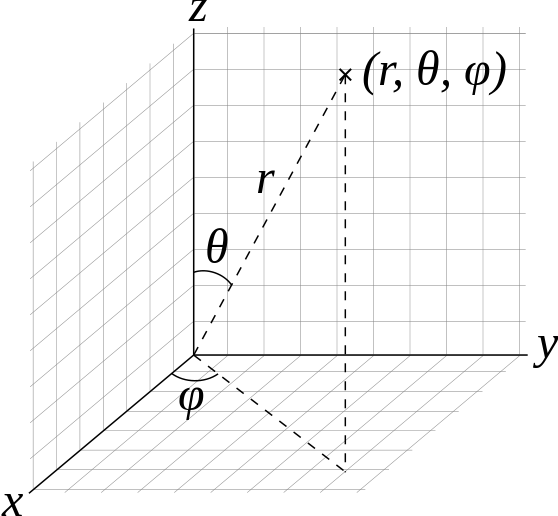
\includegraphics[width=0.5\textwidth]{Images/sphericalCoordinates.png}
	\caption{Coordenadas ésfericas}
\end{figure}
Por eso los valores esperados de los éspines nos dan
\begin{align*}
	\langle S_x \rangle = 0 \quad \Rightarrow \quad \phi = \frac{\pi}{2}
\text{o} \phi = \frac{3\pi}{2} \\
	\langle S_y \rangle = \frac{\hbar}{4} > 0 \quad \Rightarrow \quad
\phi=\frac{\pi}{2} \\
	\langle S_z \rangle > 0 \quad \Rightarrow \quad 0 < \theta < \pi
\end{align*}
Ya hemos encontrado $\phi$ y por el valor de $\theta$ vamos a utilizar el valor
esperado del éspin en la direccion y. El electron es un particular con el éspin
1/2 con que podemos utilizar los matrices de pauli $\sigma$, de que nos
conocemos el valor esperado dado por
$$
	\langle \sigma_y \rangle =\sin \theta  \sin \phi
$$
Así tenemos
\begin{align*}
	S_y &= \frac{\hbar}{2} \sigma_y \\
	\langle S_y \rangle = \frac{\hbar}{2} \langle \sigma _ y \rangle = \sin
\theta \sin \phi \overset{!}{=} \frac{\hbar}{4}
\end{align*}
Lo conocemos el valor de $\phi$ y podemos resolver la ecuacion como
$$
	2 \sin \theta \sin \frac{\phi}{2} = 1 \quad \Rightarrow \quad \sin \theta =
\frac{1}{2} \quad \Rightarrow \quad \theta = \frac{\pi}{6} = 30ª  
$$
Igualmente $\phi$ esta dado por
$$
	\phi = \frac{\pi}{2} = 90ª
$$.

\end{solucion}


